The cutting-edge of current ground-based interferometers are the twin
Advanced LIGO detectors \cite{2015CQGra..32g4001L} located in Hanford,
WA, USA, and Livingston, LA, USA. These interferometers are Michelson
interferometers with a large number of additional components, which
allow detection of differential changes in their arm lengths (strains)
on the order of $10^{-22}$.

% \begin{figure}
% \begin{adjustwidth*}{-5.5in}{-2in}
%   \centering
%   %\input{figures/interferometer.pgf}
%   \caption{An interferometer.}
%   \label{fig:interferometer}
% \end{adjustwidth*}
% \end{figure}

\subsection{Detecting gravitational waves with light}
\label{sec:interferometricdetection}

Gravitational-wave detectors which use beams of light, such as
interferometers and pulsar timing arrays rely on measuring the the
travel time of a beam of electromagnetic radiation between two points,
and the effect that a gravitational wave has on this time. A full
treatment of this is given in \cite{2009LRR....12....2S}, but in
summary, if a gravitational wave is not present within a detector, the
travel time of a beam will be constant. If a gravitational waev is
introduced, which has a polarisation component $h_+(t)$ in the plane
of the beam, the change in the arrival time of the beam will be
\begin{equation}
  \label{eq:arrival-times-gw}
  \dv{t_f}{t} = 1 + \half (1 + \cos(\theta)) \qty{ 
    h_+\qty( t + [1- \cos(\theta) ] L) - h_+(t) 
  }
\end{equation}
where $\theta$ is the angle separating the detector beam and the
gravitational wave plane, and $L$ is the proper distance separating
the clocks when no gravitational wave is present.

By arranging the detector to reflect the beam back to the originating
clock, it is possible to measure the round-triop time using only one
clock. In this arrangement we must account for the gravitational wave
having a different strength one the return trip, and so equation
(\ref{eq:arrival-times-gw}) becomes 
\begin{align}
  \label{eq:three-term}
  \dv{t~{round}}{t} = 1 + \half \Big(  (& 1-\cos(\theta) )h_+ (t+2L) - (1+\cos(\theta))h_+(t) \nonumber \\ & + 2 \cos(\theta) h_+ [t+L(1 - \cos(\theta))] \Big)
\end{align}
the \emph{three-term} relation.

\subsection{Operation of a Michelson interferometer}
\label{sec:Michelson}
%
\sidebar{
\begin{center}
  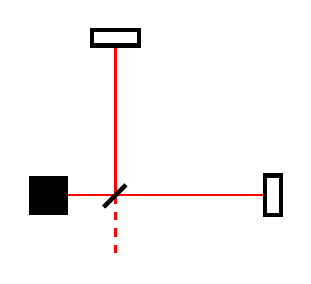
\begin{tikzpicture}
    \draw [thick, red] (0,0.25) -- (3,0.25);
    \draw [thick, red] (1.1, 0.25) -- (1.1, 2.15);
    \draw [thick, red, dashed] (1.1, 0.25) -- (1.1, -0.5);
    \fill (0,0) rectangle (0.5, 0.5);
    \draw [ultra thick] (0.95, 0.1) -- +(45:.4);
    \draw [ultra thick] (3, 0) rectangle (3.2, .5);
    \draw [ultra thick] (0.8, 2.15) rectangle (1.4, 2.35);
  \end{tikzpicture}
\end{center}
\captionof{figure}{A simple Michelson interferometer, composed of a
    light source (black box), a beam splitter (heavy black line), and
    two end mirrors (white boxes). \label{fig:michelson}}
} 
%
A Michelson interferometer is an optical device which is capable of
measuring the difference in length between two optical paths to
sub-wavelength precision. A Michelson interferometer can be
constructed using a beamsplitter and two mirrors, in the configuration
presented in figure \ref{fig:michelson}. The input beam is split along
the $x$ and $y$ directions, and reflected back to the
beam-splitter. At the beam-splitter the two beams will interfere: in
the standard Michelson setup this will result in constructive
interference if the arms have identical lengths, and a beam will be
produced at the output (the dashed red line). If the arms' relative
lengths change a pattern of interference fringes will be visible at
the output of the interferometer.

\subsection{Power Recycling}
\label{sec:power-recycling}
%
\sidebar{
\begin{center}
  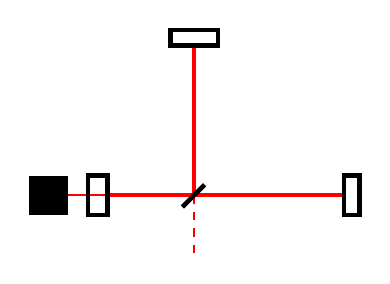
\begin{tikzpicture}
    \draw [ultra thick, red] (0,0.25) -- (3,0.25);
    \draw [ultra thick, red] (1.1, 0.25) -- (1.1, 2.15);
    \draw [thick, red] (-1,0.25) -- (0, 0.25);
    \draw [thick, red, dashed] (1.1, 0.25) -- (1.1, -0.5);
    \fill (-1,0) rectangle (-0.5, 0.5);
    \draw [ultra thick] (0.95, 0.1) -- +(45:.4);
    \draw [ultra thick] (3, 0) rectangle (3.2, .5);
    \draw [ultra thick] (0.8, 2.15) rectangle (1.4, 2.35);
    \draw [ultra thick] (-0.25, 0) rectangle (-0, 0.5);
  \end{tikzpicture}
\end{center}
\captionof{figure}{A Michelson interferometer with power recycling,
  using a comparable setup to figure \ref{fig:michelson}, but with a
  mirror added between the laser and the beam splitter. \label{fig:power-recycle}}
} 
%
The optimal signal-to-noise ratio can be achieved from an
interferometer when the arm lengths are configured so that when no
gravitational wave is present in the interferometer the interferometer
beams interfere destructively \cite{1978JPhE...11..710E}. If the
mirrors are low loss the light will then be reflected back towards the
laser, and by placing a mirror between the laser and the beam splitter
a resonant cavity can be formed (see figure \ref{fig:power-recycle}),
allowing the power in the interferometer to build up. This allows a
less powerful laser to be used as the input for the interferometer,
with a \SI{10}{\watt} laser capable of providing several kilowatts of
power inside the interferometer \cite{2011LRR....14....5P}.

\subsection{Signal Recycling}
\label{sec:signal-recycling}
%
\sidebar{
\begin{center}
  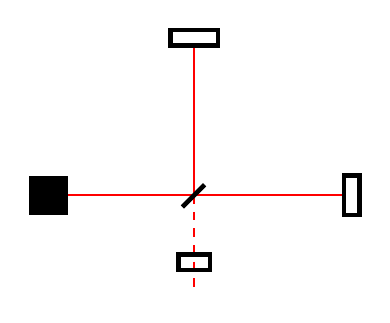
\begin{tikzpicture}
    \draw [thick, red] (0,0.25) -- (3,0.25);
    \draw [thick, red] (1.1, 0.25) -- (1.1, 2.15);
    \draw [thick, red] (-1,0.25) -- (0, 0.25);
    \draw [thick, red, dashed] (1.1, 0.25) -- (1.1, -1.0);
    \fill (-1,0) rectangle (-0.5, 0.5);
    \draw [ultra thick] (0.95, 0.1) -- +(45:.4);
    \draw [ultra thick] (3, 0) rectangle (3.2, .5);
    \draw [ultra thick] (0.8, 2.15) rectangle (1.4, 2.35);
    \draw [ultra thick] (0.9, -0.5) rectangle (1.3, -0.7);
  \end{tikzpicture}
\end{center}
\captionof{figure}{A Michelson interferometer with signal recycling,
  using a comparable setup to figure \ref{fig:michelson}, but with a
  mirror added between the output and the beam splitter. \label{fig:signal-recycle}}
} 
%
Signal recycling can be used to tune the bandwidth of an
interferometer, and to increase its sensitivity by re-injecting the
interferometer's output signal to the interferometer, achieving
resonance, which increases the signal-to-noise ratio of the
signal. This is possible thanks to the sidebands on the beam which are
produced by the gravitational wave not interfering destructively.

To perform signal recycling a mirror is added between the
beam-splitter and the readout port of the interferometer, with this
configuration illustrated in figure \ref{fig:signal-recycle}.

\subsection{Fabry-Perot Cavities}
\label{sec:fabry-perot-cavities}
%
\sidebar{
\vspace{-1cm}
\begin{center}
  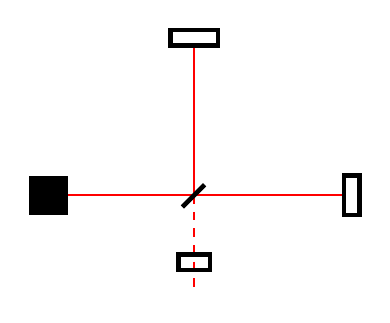
\begin{tikzpicture}
    \draw [thick, red] (0,0.25) -- (3,0.25);
    \draw [thick, red] (1.1, 0.25) -- (1.1, 2.15);
    \draw [thick, red] (-1,0.25) -- (0, 0.25);
    \draw [thick, red, dashed] (1.1, 0.25) -- (1.1, -1.0);
    \fill (-1,0) rectangle (-0.5, 0.5);
    \draw [ultra thick] (0.95, 0.1) -- +(45:.4);
    \draw [ultra thick] (3, 0) rectangle (3.2, .5);
    \draw [ultra thick] (0.8, 2.15) rectangle (1.4, 2.35);
    \draw [ultra thick] (0.9, -0.5) rectangle (1.3, -0.7);
  \end{tikzpicture}
\end{center}
\captionof{figure}{A Michelson interferometer with signal recycling,
  using a comparable setup to figure \ref{fig:signal-recycle}, but with a
  mirror added between the beam-splitter and the end mirrors of each arm. \label{fig:fabry-perot}}
}
%
The arms of modern interferometers used in the detection of
gravitational-waves store the beam for a period of time comparable to
the timescale of the signals which are being searched for. In the case
of kilometre-scale detectors and signals with a period around
\SI{1}{\milli\second} this implies the need for the light to reflect
up-and-down the detector around $50$ times. This is achieved by laying
the reflected beams atop each other in a Fabry-Perot cavity, with a
\gls{finesse}, $\mathcal{F}=50$. A Fabry-Perot cavity is formed by
placing a mirror between the beam-splitter and the end mirror in each
arm, as illustrated in figure \ref{fig:fabry-perot}.

\subsection{Advanced LIGO}
\label{sec:advanced-ligo}

The Advanced LIGO detectors are 4-kilometre long interferometers with
Fabry-Perot cavities, with a finesse of 50. The detectors improve
their sensitivity compared to the initial generation detectors through
the use of signal recycling, a technology pioneered in the GEO
detector, and have quadruple mirror suspensions which use fused silica
fibres to provide seismic
islolation\cite{2002CQGra..19.4043R,2012CQGra..29w5004A}.

%%% Local Variables: 
%%% mode: latex
%%% TeX-master: "../../document"
%%% End: 

